\section{Langkah-Langkah Percobaan}
\subsection{Persiapan Alat dan Bahan}
Sebelum memulai praktikum ini, praktikan mempersiapkan beberapa alat dan bahan yang diperlukan. Alat dan bahan yang praktikan bawa sendiri diantaranya, laptop yang sudah terinstall Winbox, dan kabel UTP. Sedangkan alat dan bahan yang telah disediakan adalah 2 set router mikrotik. Pengambilan dilakukan oleh perwakilan kelompok.

\subsection{Point to Point}
\begin{enumerate}
  \item Mereset Konfigurasi Router \\
  Sebelum memulai praktikum, praktikan mereset seluruh konfigurasi pada router. Praktikan pertama-tama membuka winbox dan login ke jaringan router. Kemudian, memilih menu system > reset configuration.
  \item Konfigurasi kabel\\
  Sebelm mengkonfigurasi router lebih jauh, praktikan menghubungkan router dan laptop sesuai topologi yang diberikan asisten praktikum. Router 2 dan 1 dihubungkan ke ether 7. Sedangkan laptop dihubungkan pada rether 6. 
  \item Konfigurasi Bridge Router 1\\
  Router 1 akan digunakan sebagai bridge. Pertama, interface ether 1 diaktifkan sebagai WLAN dengan memilih menu wireless > wifi > interface > WLAN 1. Edit konfigurasinya menajdi mode bridge dengan SSID PointToPoint\_9. Hasil dapat dilihat pada \ref{fig:ptp-router1}.
  \item Konfigurasi Router 2 \\
  Router 2 juga dikonfigurasi ether 7 nya seperti ether 1 router 1. Setelah mendapatkan interface WLAN, konfigurasinya diedit dengan nilai mode station. Setelah itu, praktikan melakukan scan untuk mendapatkan sinyal dari router 1 dengan SSID PointToPoint\_9. 
  \item Konfigurasi IP
  Terdapat 2 jenis interface yang perlu diberikan IP, yaitu interface WLAN (ether 7 router 1 dan ether 7 router 2) dan interface LAN (ether 6 router 1 dan ether 6 router 2). Praktikan melakukan konfigurasi dengan alamat seperti arahan modul. Ip laptop diset statis dengan nilai seperti di modul. Hasil dapat dilihat pada \ref{fig:ptp-ip}.
  \item Konfigurasi Routing Statis \\
  Routing ini berfungsi agar laptop bisa berkomunikasi dengan router 2. Praktikan melakukan konfigurasi routing statis pada router 1 dengan nilai Dst. Address: 192.168.30.0/24 dan Gateway: 10.10.10.2. Sedangkan pada router 2, praktikan emlakukan konfigurasi dengan nilai Dst. Address: 192.168.20.0/24 dan Gateway: 10.10.10.1. Hasil dapat dilihat pada \ref{fig:ptp-routing}.
  \item Test Koneksi
  Praktikan melakukan test koneksi dengan melakukan ping dari router ke interface WLAN router B dan dari router B ke interface WLAN router 1. Praktikan juga melakukan ping dari laptop 1 ke laptop 2 dan sebaliknya. Hasil dapat dilihat pada \ref{fig:ptp-ping}.
\end{enumerate}

\subsection{Point to Multipoint}
\begin{enumerate}
  \item Konfigurasi Interface WLAN \\
  Pada router 1, praktikan mengubah konfigurasi menjadi mode Ap Bridge dengan SSID PointToMultipoint\_9. Sedangkan pada router 2, konfigurasi WLAN diubah menjadi mode Station Bridge. Seperti sebelumnya, pada router 2 praktikan melakukan scan untuk mendapatkan koneksi ke router 1 melalui SSID PointToMultipoint\_9. Hasil dapat dilihat pada \ref{fig:ptm-konfigure}.
  \item Konfigurasi IP dan Routing Statis\\
  Karena praktikan tidak emlakukan reset, maka praktikan tidak perlu mengeset IP lagi.
  \item Test Koneksi \\
  Praktikan melakukan test koneksi dengan melakukan ping dari router ke interface WLAN router B dan dari router B ke interface WLAN router 1. Praktikan juga melakukan ping dari laptop 1 ke laptop 2 dan sebaliknya. Hasil dapat dilihat pada \ref{fig:ptm-ping}.
\end{enumerate}

\subsection{Bridge}
\begin{enumerate}
  \item Konfigurasi Interface LAN \\
  Pada router 1, konfigurasi WLAN diubah menajdi Bridge dengan SSID WirelessBridge\_9. Sedangkan pada router 2 diubah menjadi mode station pseudobridge. Setelah itu, pada router 2 praktikan melakukan scan untuk terhubung dengan SSID WirelessBridge\_9. Hasil dapat dilihat pada \ref{fig:wb-konfigure}.
  \item Konfigurasi IP dan Routing Statis\\
  Karena praktikan tidak emlakukan reset, maka praktikan tidak perlu mengeset IP lagi. Routing statis dihapus
  \item Membuat Bridge \\
  Brige bertujuan untuk langsung mengalihkan koneksi ke port atau interface tertentu tanpa routing. Pada oruter 1 dan 2, praktikan masuk ke menu Bridge > + dan diberi nama bridge1. ada menu Bridge > Ports, praktikan menambahkan konfigurasi untuk WLAN router 1 dan ether 7 router 2 agar terhubung dengan bridge1.
  \item Test Koneksi \\
  Praktikan melakukan test koneksi dengan melakukan ping dari router ke interface WLAN router B dan dari router B ke interface WLAN router 1. Praktikan juga melakukan ping dari laptop 1 ke laptop 2 dan sebaliknya. Hasil dapat dilihat pada \ref{fig:wb-ping}.
\end{enumerate}

\section{Analisis Hasil Percobaan}
Praktikum pertama koneksi Point To Point, praktikan belajar memahami bagaimana cara kerja suatu router dalam memberikan access point tunggal. Pad percobaan ini router berperan sebagai WiFi Transmitter. Pad percobaan ini, praktikan berhasil menghubungkan WLAN router 1 dan router 2 sehingga koneksi berhasil terjadi. Percobaan kedua koneksi Point To Multipoint, praktikan belajar memahami bagaimana souter dapat memberikan koneksi kepada lebih dari satu point (multipoint). Pada ercobaan ini, praktikan berhasil melakukan koneksi dari laptop 1 ke laptop 2 dan sebaliknya yang berada  di subnet yang sama. Pada percobaan pertama dna kedua ini, router berfungsi sebagai router biasa dengan tambahan kemampuan wireless. Oleh karena itu, agar laptop 1 dan laptop 2 dapat berkomunikasi, masih diperlukan routing (dalam percobaan ini dilakukan secara statis). Hal ini sesuai dengan teori kalau pada subnet yang berbeda, diperlukan routing agar perangkat pada kedua subnet ini bisa berkomunikasi. Percobaan kedtiga praktikan mencoba penggunaan wireless bridge. Praktikan berhasil melakukan konfigurasi dan melakukan komunikasi antar laptop. Berbeda dnegan dua percobaan pertama, percobaan ini tidak menggunakan routing karena router berfungsi sebagai bridge atau switch secara fungsi. Sebagaimanateroi, bahwa pada switch perangkat yang terhubung dianggap berada di network yang sama.

\section{Hasil Tugas Modul}
Simulasikan jaringan wireless antara tiga gedung:
\begin{itemize}
  \item Gedung Pusat
  \item Gedung Lab
  \item Gedung Asrama (Hubungkan dua bagian dalam Gedung Asrama (Blok A dan Blok B) menggunakan Wireless Bridge Point-to-Point.)
\end{itemize}
Menggunakan Point-to-Multipoint (PTMP) di Cisco Packet Tracer. \\

Berikut ini merupakan hasil dari simulasi. File dapat di cek di tumod > tumod jarkom p3.pkt
\begin{figure}[htbp]
    \centering
    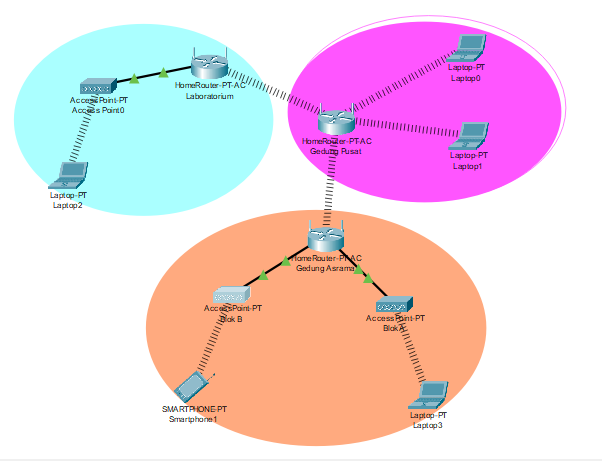
\includegraphics[width=0.5\linewidth]{tumod/tumod jarkom3.png} 
    \caption{Hasil Simulasi Tugas Modul}
    \label{fig:tumod}
\end{figure}



\section{Kesimpulan}
Berdasarkan percobaan yang telah dilakukan, dapat diambil beberapa kesimpulan penting. Pertama, router yang mendukung adanya koneksi wireless dapat memberikan koneksi secara point to point maupun point to multipoint. Kedua, walaupun koneksi dilakukan secara wireless, tetap dibutuhkan routing agar perangkat bisa saling berkomunikasi. Ketiga, ketika router digunakan sebagai switch (bridge) router tetap bisa menggunakan fungsionalitas wireless nya.

\section{Lampiran}
\subsection{Dokumentasi saat praktikum}
\begin{figure}[htbp]
    \centering
    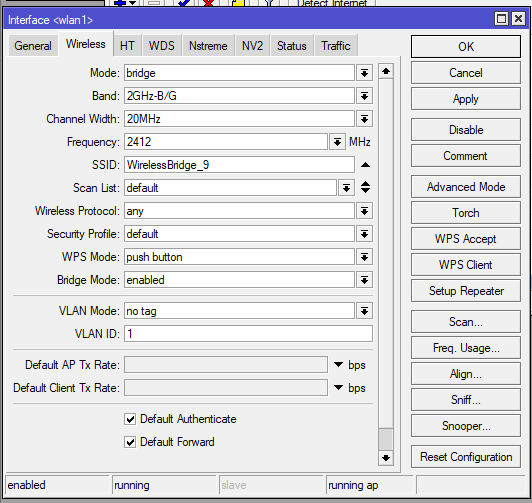
\includegraphics[width=0.5\linewidth]{dokum/Laptop 1/bridge.png} 
    \caption{Hasil Konfigurasi WLAN}
    \label{fig:ptp-router1}
\end{figure}

\begin{figure}[htbp]
    \centering
    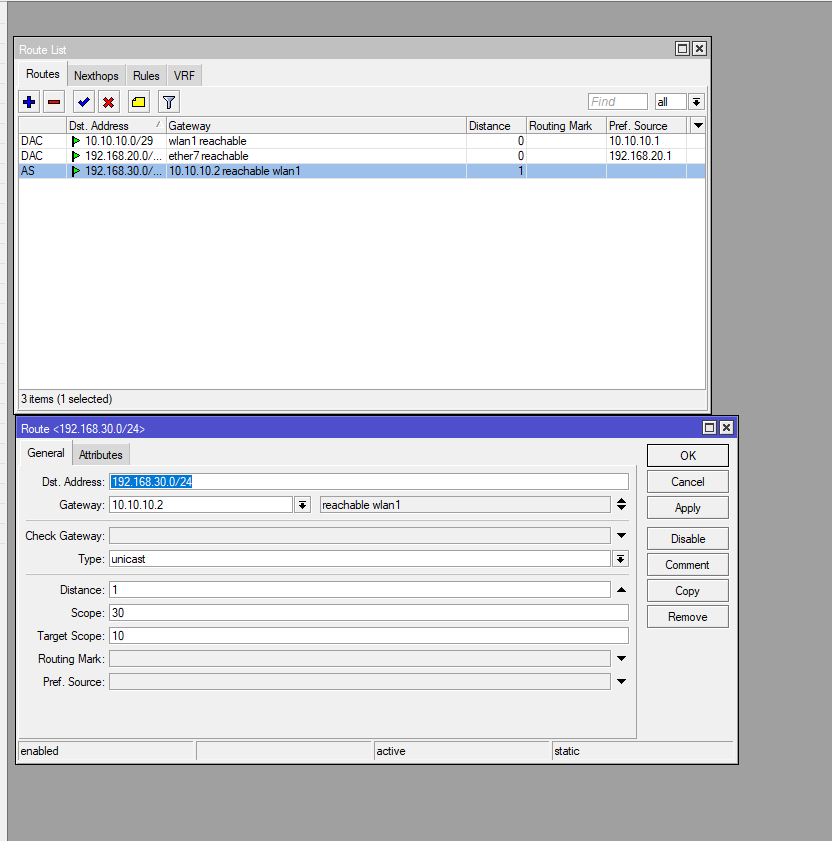
\includegraphics[width=0.5\linewidth]{dokum/Laptop 1/ptp ip.png} 
    \caption{Hasil IP}
    \label{fig:ptp-ip}
\end{figure}

\begin{figure}[htbp]
    \centering
    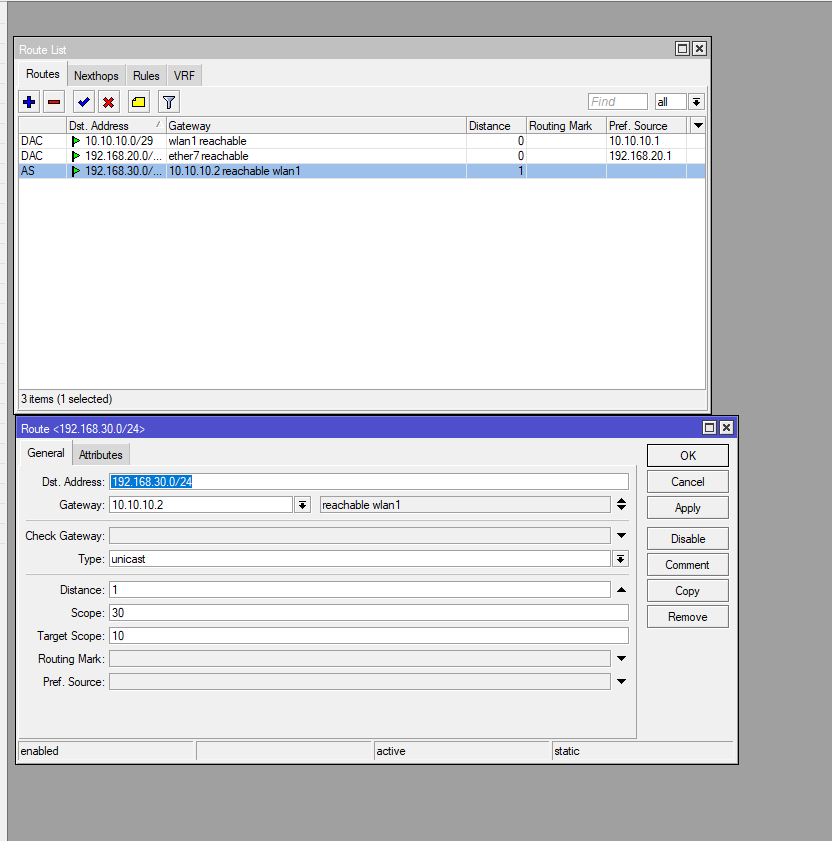
\includegraphics[width=0.5\linewidth]{dokum/Laptop 1/routes wlan router a.png} 
    \caption{Hasil Routing}
    \label{fig:ptp-routing}
\end{figure}

\begin{figure}[htbp]
    \centering
    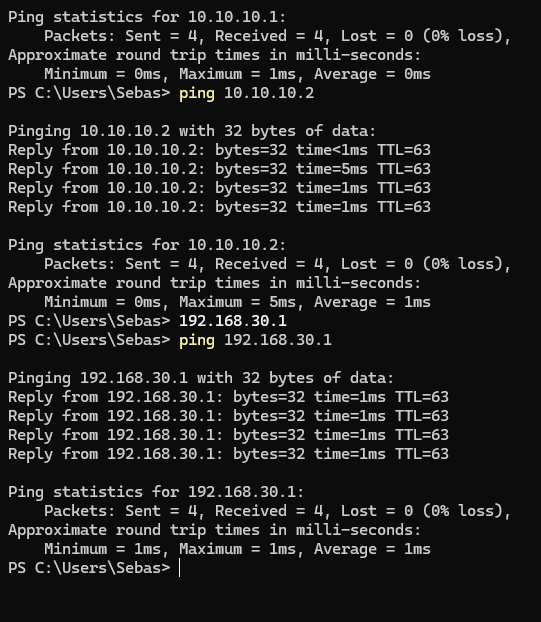
\includegraphics[width=0.5\linewidth]{dokum/Laptop 1/ping ptp.png} 
    \caption{Hasil Ping}
    \label{fig:ptp-ping}
\end{figure}

\begin{figure}[htbp]
    \centering
    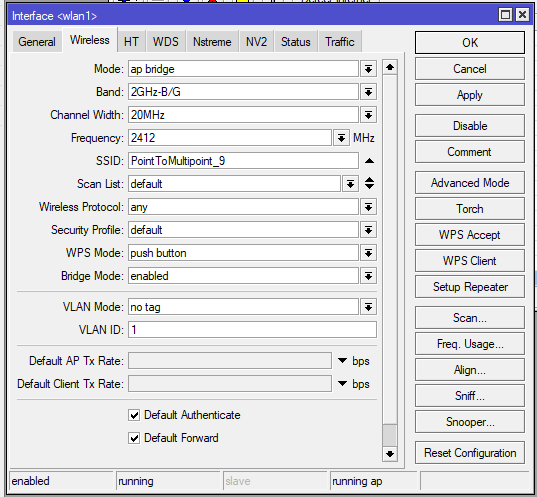
\includegraphics[width=0.5\linewidth]{dokum/Laptop 1/jarkom3-ptm-awt interfaces.png} 
    \caption{Hasil Konfigurasi PTM}
    \label{fig:ptm-konfigure}
\end{figure}

\begin{figure}[htbp]
    \centering
    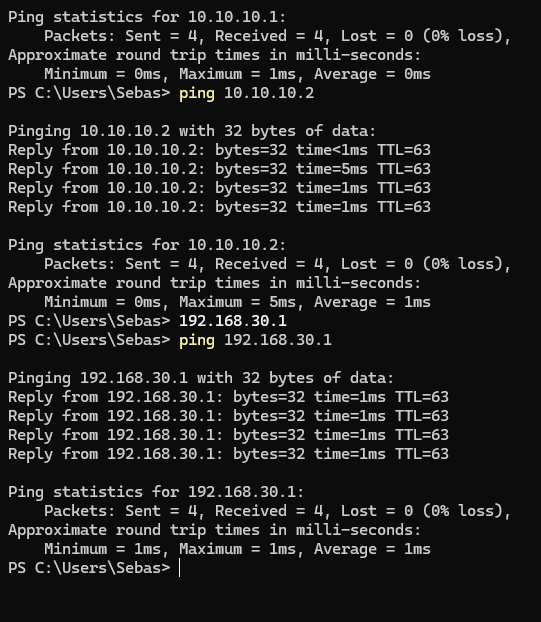
\includegraphics[width=0.5\linewidth]{dokum/Laptop 1/jarkom3-ptm-ping.png} 
    \caption{Hasil Ping PTM}
    \label{fig:ptm-ping}
\end{figure}

\begin{figure}[htbp]
    \centering
    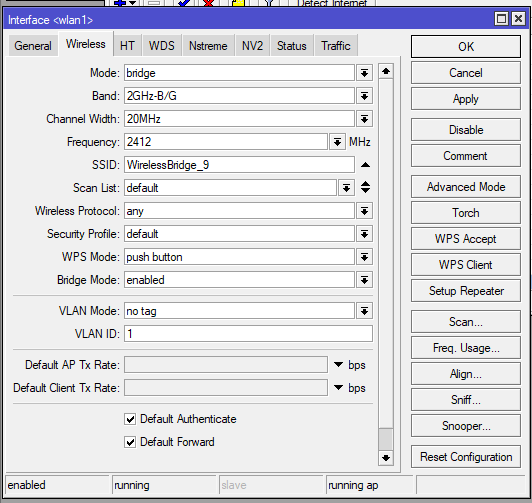
\includegraphics[width=0.5\linewidth]{dokum/Laptop 1/jarkom3-wb-interfaces.png} 
    \caption{Hasil Konfigurasi WB}
    \label{fig:wb-konfigure}
\end{figure}

\begin{figure}[htbp]
    \centering
    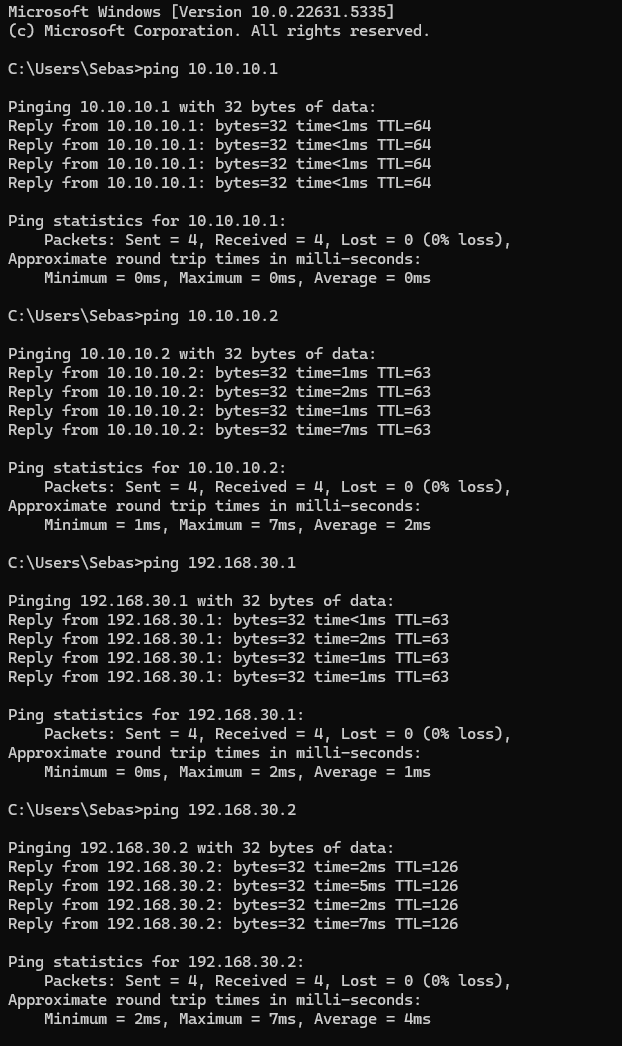
\includegraphics[width=0.5\linewidth]{dokum/Laptop 1/jarkom3-wb-ping.png} 
    \caption{Hasil Ping WB}
    \label{fig:wb-ping}
\end{figure}

\begin{figure}[htbp]
    \centering
    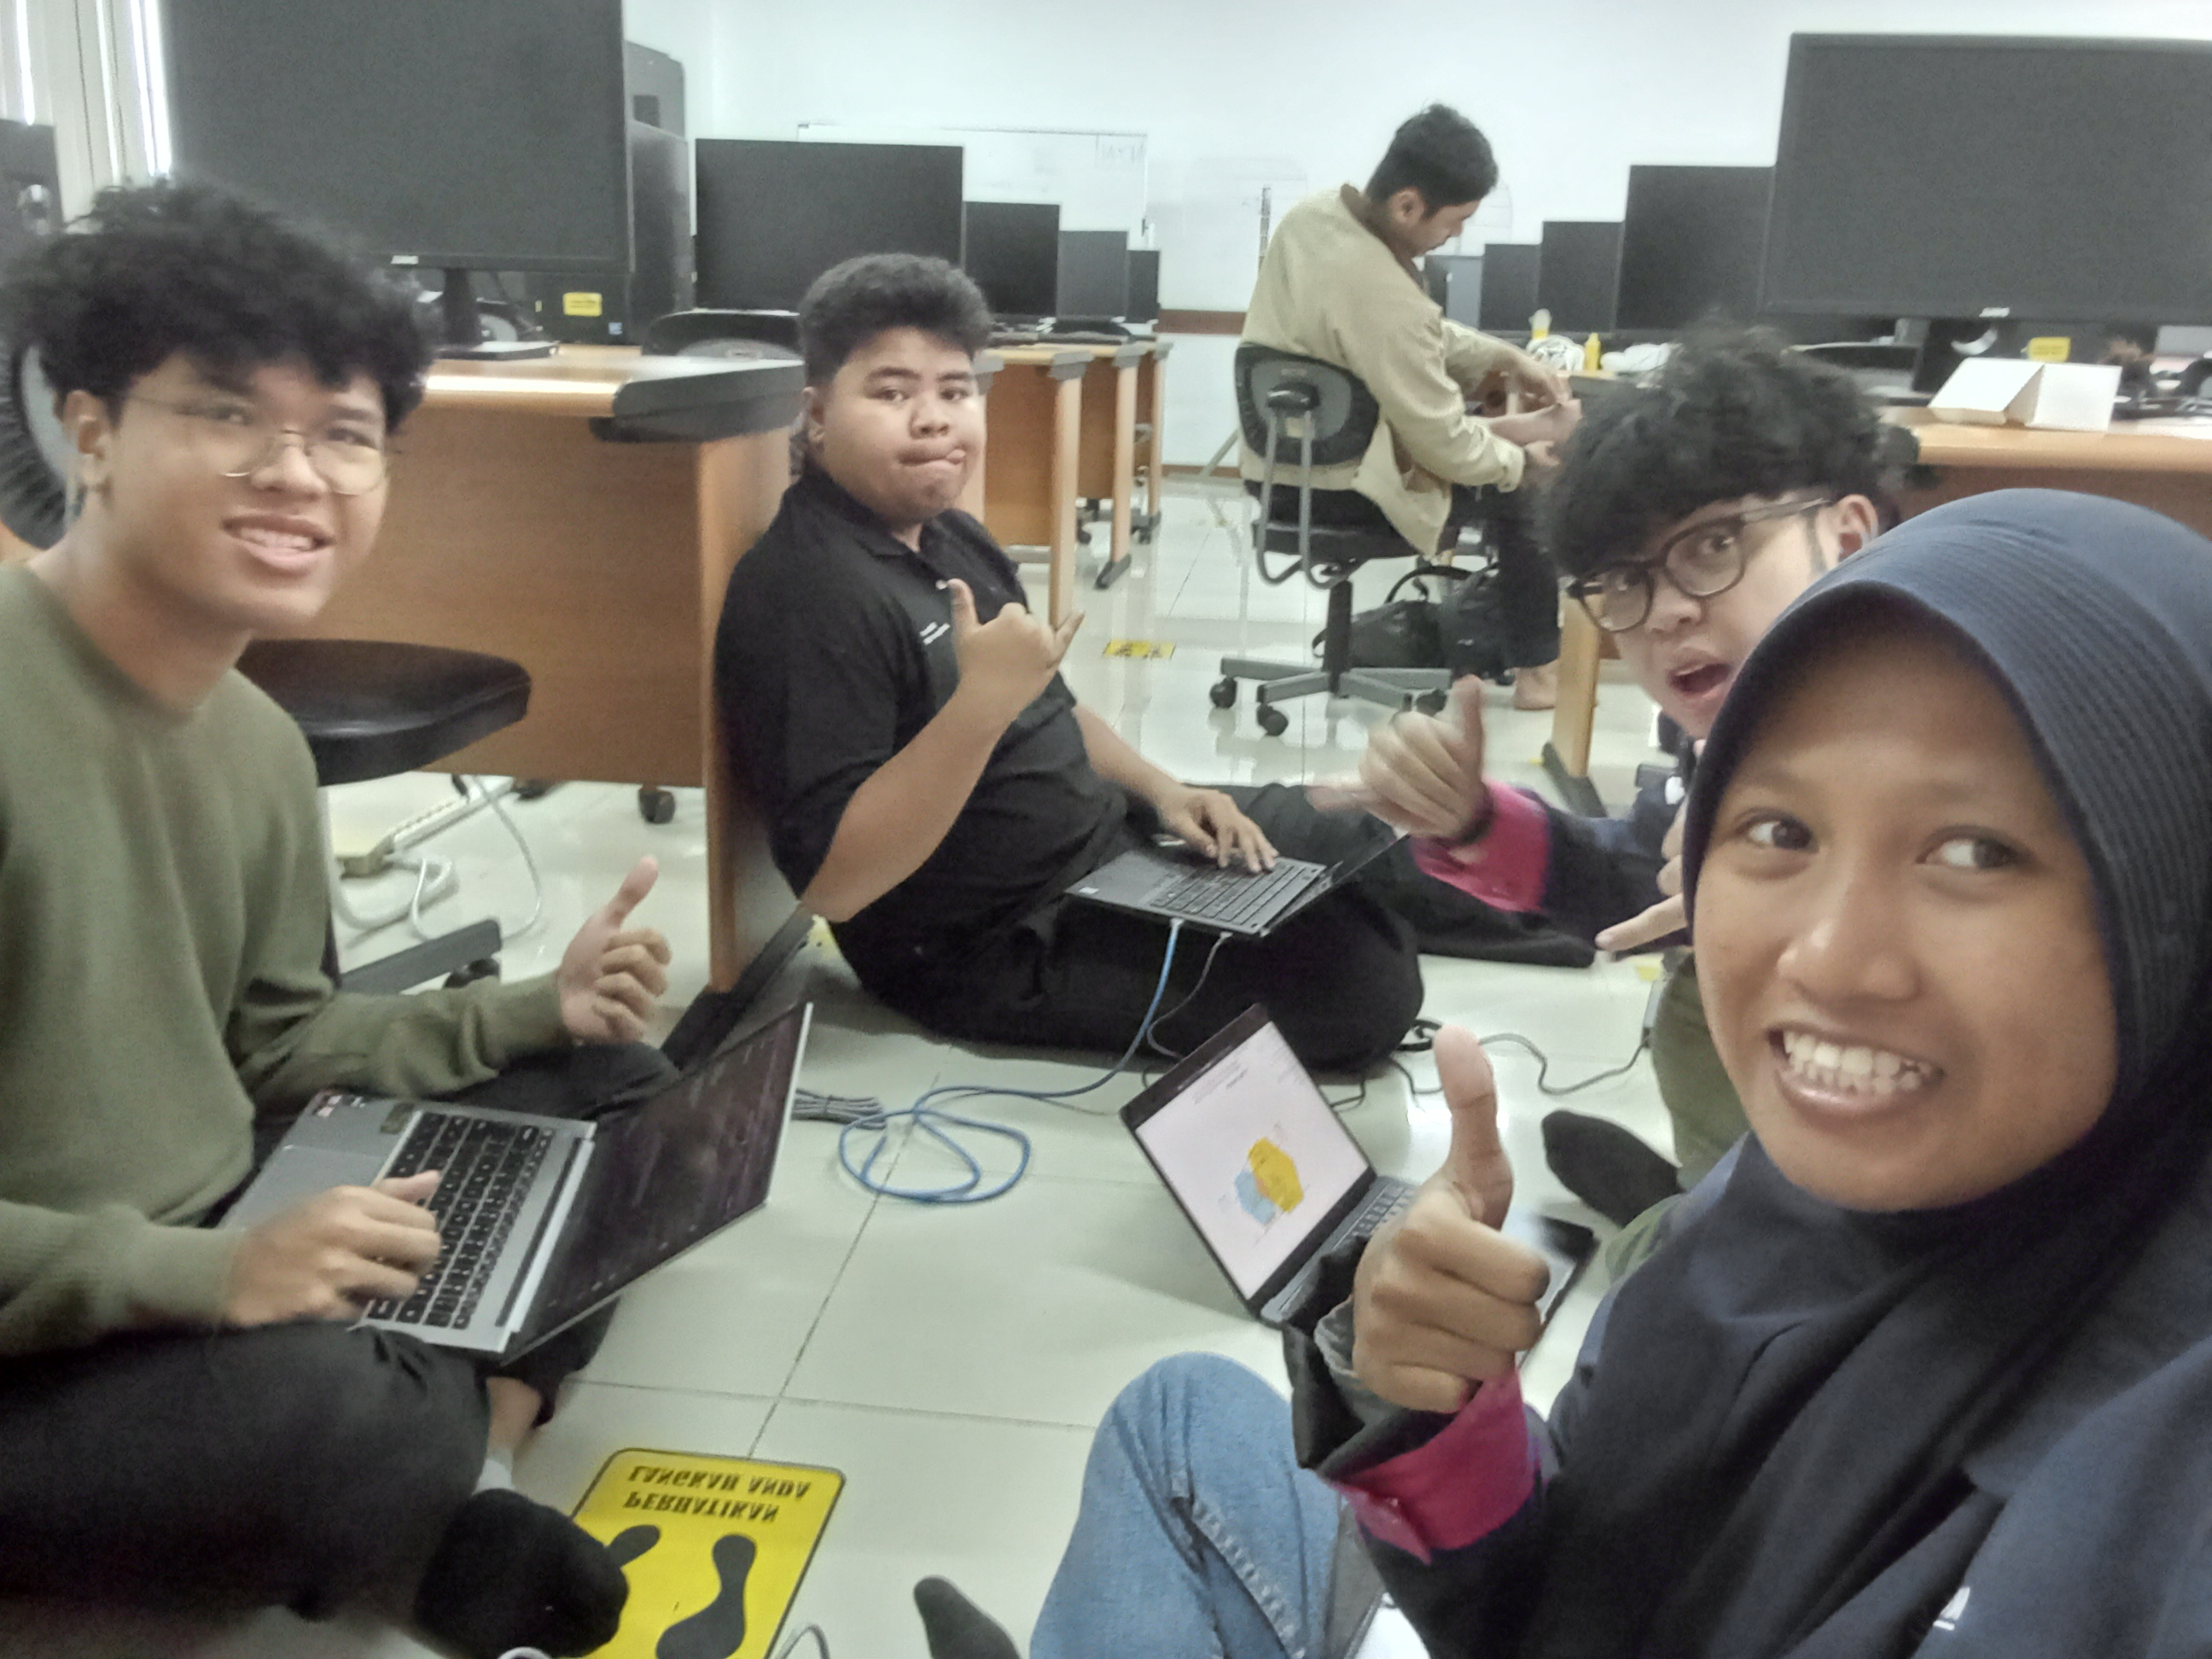
\includegraphics[width=0.5\linewidth]{dokum/IMG20250524100735.jpg} 
    \caption{Dokumentasi}
    \label{fig:dokumentasi}
\end{figure}
